\chapter{Particle Identification}
\section{Radiazione Cherenkov}
L'effetto Cherenkov si ha quando una particella attraversa un mezzo con velocità superiore a quella della luce nel mezzo stesso ($c_n=c_0/n$).
\\ \\ 
La radiazione Cherenkov è causata dalla polarizzazione asimmetrica del mezzo al passaggio della particella che, rilassandosi e tornando all'equilibrio, genera una radiazione di dipolo (questo succede per ogni sezione infinitesima della traccia della particella)

\begin{figure}[H]
    \centering
    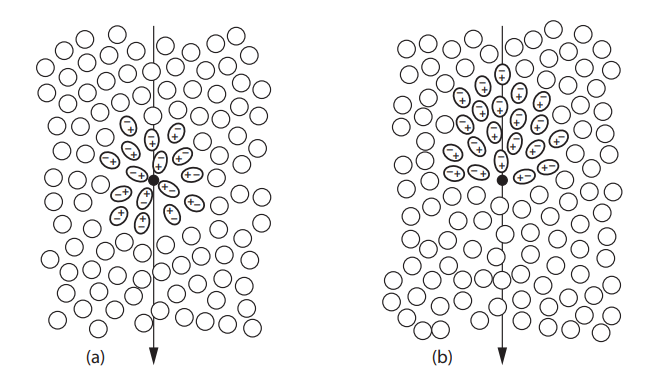
\includegraphics[width=0.7\textwidth,frame]{Chapters/images/Particle_identification/image-20220316192558631.png}
    \captionsetup{width=0.7\textwidth}
    \caption{A: Una particella a bassa velocità polarizza il mezzo in modo simmetrico\\ \\ B: A velocità superiori a quella della luce nel mezzo la polarizzazione diventa fortemente asimmetrica}
    \label{fig:}
\end{figure}

\hspace{-20pt}
\begin{minipage}{0.6\textwidth}
    \begin{figure}[H]
        \centering
        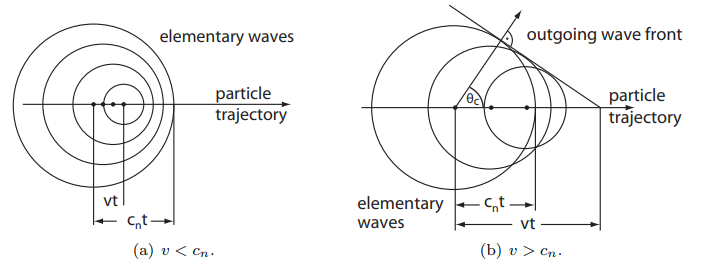
\includegraphics[width=\textwidth,frame]{Chapters/images/Particle_identification/image-20220316193152123.png}
        \captionsetup{width=\textwidth}
        \caption{Da questa figura si può ricavare facilmente l'angolo Cherenkov}
        \label{fig:}
    \end{figure}
\end{minipage} \hspace{5pt}
\begin{minipage}{0.35\textwidth}

    Ogni punto della traccia genera un'onda e se la particella ha $v>c_n$ (con $c_n$ velocità di fase della luce nel mezzo) queste onde interferiscono in modo costruttivo

\end{minipage}
L'emissione Cherenkov avviene ad un angolo fissato che aumenta con la velocità della particella
\[\cos(\theta_C)=\frac{1}{\beta n}\]
\begin{note}[Rinculo]
    Il rinculo causato dall'emissione del fotone è trascurata ma calcoli in QM mostrano che questa approssimazione è valida nella maggior parte dei casi

\end{note}
Questo angolo se misurato può subire uno \textbf{smearing}  dovuto alla relazione di dispersione del mezzo che non è costante nella frequenza

\begin{tcolorbox}[colback=NavyBlue!5]
\textbf{Recap}: La radiazione Cherenkov avviene se:
\begin{itemize}
    \item La particella ha velocità maggiore alla velocità di fase nel mezzo alla data frequenza di emissione (poichè per relazione di dispersione $n=n(\omega)$)
\item Il mezzo è trasparente nell'ottico e ha dimensioni superiori alla linghezza d'onda della radiazione (necessario per permettere l'interferenza costruttiva)

\end{itemize}

Inoltre, a una distanza sufficiente dalla traccia della particella, le onde hanno polarizzazione trasversa: sono polarizzate linearmente in un piano contenente la direzione di propagazione dell'onda e la traccia della particella
\end{tcolorbox}

\subsection{Cherenkov Threshold}
La \textbf{velocità minima}  per cui si ha emissione Cherenkov si ottiene ponendo $\cos(\theta_C)=1$ (Ovvero emissione in avanti a $0°$)
\[\beta_\text{th}=\frac{1}{n}\]
All'aumentare di $\beta$ cresce sia l'angolo che l'intensità dell'emissione.\\ 
L'\textbf{angolo massimo}  invece si ottiene per $\beta=1$
\[\begin{gathered}
    \cos(\theta_\text{max})=\frac{1}{n}
\\ 
\sin\theta_\text{max}=\sqrt{1-\cos(\theta_\text{max})^2}=\sqrt{1-\frac{1}{n^2}}=\frac{1}{\gamma_\text{th}}
\end{gathered}\]

\hspace{-10pt}
\begin{minipage}{0.6\textwidth}
    
    \begin{figure}[H]
        \centering
        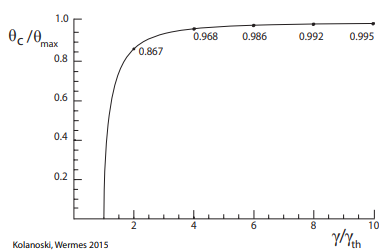
\includegraphics[width=1.01\textwidth,frame]{Chapters/images/Particle_identification/image-20220317114142322.png}
    \end{figure}
\end{minipage} \hspace{5pt}
\begin{minipage}{0.41\textwidth}
\vspace{9pt}
    \begin{figure}[H]
        \captionsetup{width=\textwidth}
        \caption{Facendo il plot dell'angolo cherenkov normalizzato in funzione del $\gamma$ (normalizzato) si nota come il range di sensibilità di un rivelatore cherenkov è molto stretto dato che oltre una certa velocità la variazione dell'angolo di emissione è quasi nulla.\\ Già a $\gamma=2 \gamma_\text{th}$ l'angolo cherenkov ha raggiunto l'87\% del suo valore asintotico $\theta_\text{max}$}
    \end{figure}


\end{minipage}
Con semplici conti è possibile esprimere il seno dell'angolo in funzione di gamma
\[\begin{gathered}
    \sin^2(\theta_C)=\sin^2(\theta_\text{max})\frac{\gamma^2-\gamma_\text{th}^2}{\gamma^2-1} \implies
\\ 
\implies \lim_{\gamma \to \infty} \frac{\theta_c}{\theta_\text{max}} \simeq \frac{R_c}{R_\text{max}} \simeq \sqrt{1-\frac{\gamma_\text{th}^2}{\gamma^2}}
\end{gathered}\]
dove $R_c$ ed $R_\text{max}$ sono i raggi dei rispettivi anelli cherenkov.

\subsection{Spettro di emissione}
\begin{theorem*}[Formula di Frank-Tamm] \hfill \\ 
    Si ha radiazione Cherenkov solo per $\beta ^{2} n^{2} (\omega )>1$ e lo spettro è:
    \[\frac{d^{2}  E}{ d\omega  \: dx}  = \frac{z^{2} e^{2} }{4\pi \epsilon _{0} c^{2} }\omega \mathexplain[cd]{\left( 1-\frac{1}{\beta ^{2} n^{2}(\omega ) } \right)}{\sin ^{2} \theta _{c} (\omega )}  \]
\end{theorem*}

\begin{remark} \hfill \\
    \vspace{-20pt}
    \begin{itemize}
        \item \textbf{Si noti la linearità nella frequenza} 
        \item Le perdite di energia per luce Cherenkov sono già inluse nella Bethe Bloch ma sono largamente trascurabili: costituiscono meno dell'1\% della perdita di energia nei materiali pesanti e possono arrivare al massimo al 5\% nei gas leggeri
    \end{itemize}


\end{remark}
Un semplice modello per la permittività del mezzo è dato dalla semplice somma sulle sue frequenze di risonanza trascuranto i termini di smorzamento
\[\epsilon(\omega)=1+\frac{n_ae^2}{\epsilon_0m_e}\sum_i \frac{f_i}{\omega_{0i}^2-\omega^2}\]
con $n_a$ densità degli atomi e $f_i$ ampiezza relativa alla frequenza di risonanza i-esima con normalizzazione $\sum_i f_i=Z$.
\begin{note} 
    Ovviamente trattando gli elettroni come oscillatori senza smorzamento si ottiene una divergenza non fisica

\end{note}



\hspace{-15pt}
\begin{minipage}{0.48\textwidth}
    \begin{figure}[H]
        \centering
        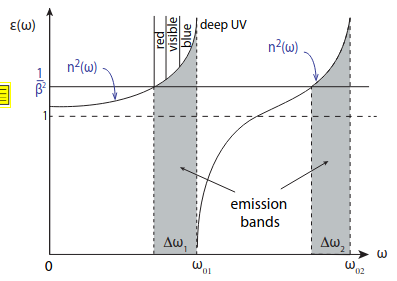
\includegraphics[width=\textwidth,frame]{Chapters/images/Particle_identification/image-20220317143923078.png}
        \captionsetup{width=\textwidth}
        \caption{Poichè l'emissione avviene solo per $n^2>\frac{1}{\beta^2}$ da plot di questo tipo possiamo individuare le bande di frequenze $\Delta \omega_i$ in cui avviene l'emissione}
    \end{figure}
\end{minipage} \hspace{5pt}
\begin{minipage}{0.48\textwidth}

    Inoltre, per materiali non magnetici ($\mu \sim 1$) vale $n(\omega)\sim\sqrt{\epsilon(\omega)}$\\ 
(In realtà $\epsilon$ ha anche una parte immaginaria che causa assorbimento)
\begin{details}["Fun" fact]\hfill \\
    Il fatto che nelle vasche di raffreddamento delle centrali nucleari si veda luce blu è dovuto sia al fatto che lo spettro Cherenkov è più spostato sul blu, sia al fatto che per scattering raylight la luce a frequenza maggiore viene diffusa maggiormente, sia all'assorbimento della luce a più bassa frequenza, sia alla curva di risposta dell'occhio umani

\end{details}
    

\end{minipage}

\begin{figure}[H]
    \centering
    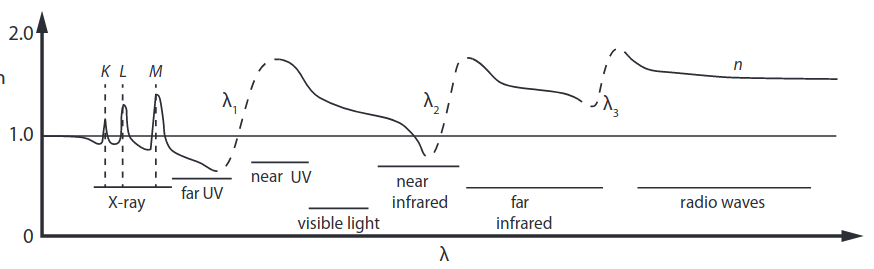
\includegraphics[width=0.95\textwidth,frame]{Chapters/images/Particle_identification/image-20220317154755537.png}
    \captionsetup{width=0.95\textwidth}
    \caption{Le linee tratteggiate rappresentano le zone di dispersione anomala\\ Per un mezzo reale trasparente nell'ottico sono presenti anche:\\-  zone a $n<1$ in cui non si può avere emissione. \\- Bande di emissione nell'infrarosso e nel radio (e anche a energie quasi discrete nella regione degli X)}
    \label{fig:}
\end{figure}

\sssec{Spettro dei singoli fotoni}
Dividendo la formula di Frank Tamm per l'energia di un singolo fotone $E=\hbar \omega$ si ottiene
\[\frac{d^2N}{dEdx}= \frac{\alpha}{\hbar c}z^2\left( 1-\frac{1}{\beta^2n^2(\omega)} \right) \xrightarrow{z=1} \; \sim 370 \sin^2(\theta_C)/eV/cm\]
con $\alpha=e^2/(4\pi \epsilon_0 \hbar c)$
\begin{note} questa equazione non ha nulla di quantistico, è stato inserito un $\hbar$ solo perchè si è scelto di raggruppare tutte le costanti con la costante di struttura fine

\end{note}
Usando la relazione $\omega=2\pi c / \lambda$ otteniamo
\[
\frac{d^2N}{d\lambda dx}=\frac{2\pi z^2 \alpha}{\lambda^2}\sin^2(\theta_c(\lambda))\]

\begin{remark}\hfill \\
    Quindi lo spettro $\frac{dN}{d\omega}=Const.$ mentre $\frac{dN}{d\lambda}\propto\frac{1}{\lambda^2}$
\end{remark}
Integrando su $x$, data L la lunghezza del mezzo, si ha
\[\frac{dN}{d\lambda}=\frac{2\pi z^2 \alpha}{\lambda^2}L\sin^2(\theta_c(\lambda)) \xrightarrow{\lambda \to \infty}\frac{2\pi z^2 \alpha}{\lambda^2}\frac{L}{\gamma_\text{th}^2}
\]
\hspace{-5pt}
\begin{minipage}{0.65\textwidth}
    \begin{figure}[H]
        \centering
        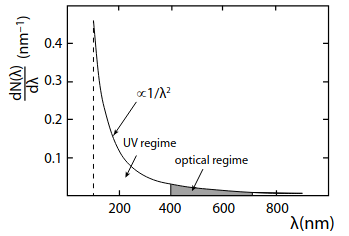
\includegraphics[width=\textwidth,frame]{Chapters/images/Particle_identification/image-20220317171549887.png}

    \end{figure}
\end{minipage} \hspace{5pt}
\begin{minipage}{0.35\textwidth}
\begin{figure}[H]
    \centering
    \captionsetup{width=\textwidth}
    \caption{Dipendenza dalla lunghezza d'onda dello spettro cherenkov. \\ Nell'UV c'è un cutoff dovuto alla dispersione anomala del mezzo}
\end{figure}
    

\end{minipage}

\sssec{Photon Yield}
Per ottenere il numero di fotoni ottici emessi integriamo lo spettro nella regione ottica.
Assumendo $n$ (e quindi $\theta_c$) costante nella regione ottica abbiamo
\[N_\text{opt}=z^2L\sin^2(\theta_c)\int_{400nm}^{700nm}\frac{2\pi \alpha}{\lambda^2}d\lambda\simeq z^2L\sin^2(\theta_c) \cdot \left(491 \frac{\text{ photons}}{cm}\right)\]

Quindi, soprattutto nel caso di indici di rifrazione molto bassi, il numero di fotoni può essere molto basso (spesso ci si ritrova a dover ricostruire anelli con 10 fotoni)
\\ 
Il numero di \textbf{fotoelettroni}  dipende anche da T($\lambda$): trasmittanza della finestra del dector, Q($\lambda$): efficienza quantica, R($\lambda$): riflettività degli specchi usati per focalizzare i fotoni sul detector
\[N_{pe}=2 \pi \alpha z^2 L \sin^2(\theta_c)\int_{\lambda_{1}}^{\lambda_{2}}T(\lambda)\: Q(\lambda) \: R(\lambda) \: \frac{1}{\lambda^2}d\lambda\]
\begin{details}\hfill \\
    \textit{L'integrale è chiamato figure of merit e caratterizza totalmente la risposta del detector } \\ 
    Valori tipici per il prodotto delle 3 funzioni di risposta sono intorno al 30\% ($Q\sim0.4$ , $T\sim0.8$,  $R\sim1$) quindi solitamente $N_{pe}\sim L \sin^2(\theta_c) \cdot150 (\text{photons}/cm)$
\end{details}
Anche qui è possibile normalizzare il numero di fotoni rispetto il caso asintotico (effettuando l'appossimazione $\sin(\theta_c)\sim \theta_c$)
\[\frac{N_\gamma}{N_\infty}\sim\frac{\theta_c^2}{\theta^2_\text{max}}\sim1-\frac{\gamma^2_\text{th}}{\gamma^2}\]

\begin{figure}[H]
    \centering
    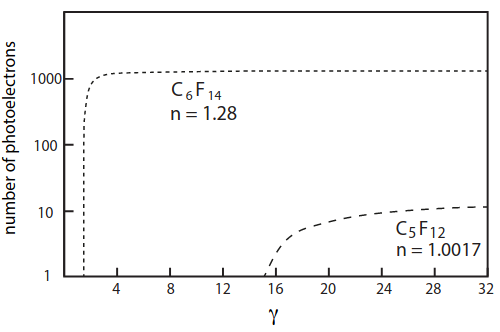
\includegraphics[width=0.7\textwidth,frame]{Chapters/images/Particle_identification/image-20220317174427644.png}
    \captionsetup{width=0.7\textwidth}
    \caption{Numero di fotoelettroni in funzione di $\gamma$ per diversi materiali con $L=20cm$ e $ Q \cdot T \cdot R \sim 0.35$}
    \label{fig:}
\end{figure}

\subsection{Tipi di detector Cherenkov}
L'effetto cherenkov può essere sfruttato in diversi modi:
\begin{itemize}
    \item Threshold: seleziona solo particelle al di sopra di una certa velocità
\item Time of Flight
\item Particle identification
\item Misura di $\beta$ (e se impulso noto da altri detector anche massa)
\end{itemize}

\sssec{Threshold}



\begin{minipage}{0.4\textwidth}
    \begin{figure}[H]
        \centering
        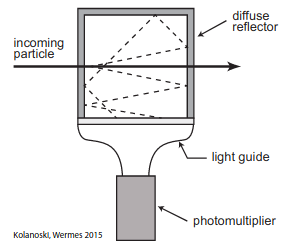
\includegraphics[width=\textwidth,frame]{Chapters/images/Particle_identification/image-20220317181632663.png}

    \end{figure}
\end{minipage} \hspace{10pt}
\begin{minipage}{0.55\textwidth}

    In questi detector non viene misurato l'angolo Cherenkov e si ha solo una risposta si/no.\\ 
    L'impulso di soglia è $p_\text{th}=mc^2(\beta \gamma)_\text{th}=\frac{mc^2}{\sqrt{n^2-1}}$
Se il momento è noto da altri detector (spesso sfruttando un cambo magnetico) si  può usare il detector cherenkov come soglia sulla massa $m_{th}c^2=p\sqrt{n^2-1}$

\begin{details}
    
    Spesso come mezzo viene usato un gas in quanto è possibile modificare $n$, e quindi la soglia, al variare della pressione del gas

\end{details}
\end{minipage}
Se vogliamo osservare un range di energia troppo grande conviene usare più detector in successione con threshold crescente in modo tale che i detector si "accendono" in sequenza e misurando l'impulso è possibile fare \textbf{PID} 

\begin{figure}[H]
    \centering
    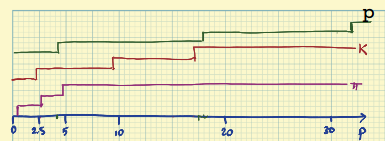
\includegraphics[width=0.8\textwidth,frame]{Chapters/images/Particle_identification/image-20220317185548344.png}
    \captionsetup{width=0.8\textwidth}
    \caption{Particle identification con 3 detector Cherenkov a threshold}
    \label{fig:}
\end{figure}

\begin{note}
    $\theta_c$ non viene misurato nei threshold counter

\end{note}
\vspace{-10pt}
\paragraph*{Risoluzione di un threshold detector}
Volendo si può fare particle identification con questi detector misurando il numero di fotoni emessi.
\\ 
L'incertezza legata al numero di fotoni è
 $\sigma_N=\frac{\partial N}{\partial \theta_c}\sigma_{\theta_c}=\frac{2N}{\tan(\theta_c)}\sigma_{\theta_c}= \sqrt{N}$ dove $\sigma(\theta_c)$ è lo spread angolare che varia con $\beta$
 \begin{details}
    \begin{itemize}
        \item Dopo quella derivata si è moltiplicato e diviso per $\sin(\theta_c)$ per riscrivere il numero di fotoelettroni e la tangente
        \item $\sigma_N=\sqrt{N}$ poichè statistica sui conteggi è poissoniana

    \end{itemize}
 
 \end{details}
 La risoluzione su $\beta$ invece è  (usando $\beta=1/(n \cos(\theta_c))$)
$\sigma_\beta=\frac{\partial \beta}{\partial \theta_c} \; \sigma_{\theta_c}=\beta \tan(\theta_c)$
\\ 
Quindi mettendo tutto insieme si tronva $\frac{\sigma_\beta}{\beta}=\frac{\tan^2(\theta_c)}{1\sqrt{N}}$

\sssec{RICH (Ring Imaging Cherenkov Detector)}